\documentclass{article}
\usepackage[usenames]{color} %used for font color
\usepackage{amssymb} %maths
\usepackage{amsmath} %maths
\usepackage[utf8]{inputenc} %useful to type directly diacritic characters
%\usepackage[linesnumbered,ruled,vlined]{algorithm2e}
\addtolength{\topmargin}{-.975in}
%\pagenumbering{gobble}
\usepackage{url}
%\usepackage{hyperref}
\usepackage{float}
\usepackage{pgfplots}
\usepackage{tikz}
\usepackage{graphicx}
\usepackage[french]{babel}




\title{Second Rapport INF6404A : Présentation du Middleware}
\author{
	Alexandre Mao\\
	David Johannès \\
	Philippe Troclet \\
	Fabien Berquez \\
	D\'{e}partement G\'{e}nie Informatique et G\'{e}nie Logiciel \\
	\'{E}cole Polytechnique de Montr\'{e}al, Qu\'{e}bec, Canada \\
	\texttt{alexandre.mao@polymtl.ca}\\
	\texttt{david.johannes@polymtl.ca}\\
	\texttt{philippe.troclet@polymtl.ca}   \\
	\texttt{fabien.berquez@polymtl.ca}   \\
}
\date{19 mai 2016}

\usepackage{natbib}
\usepackage{graphicx}

\begin{document}

\maketitle

\section{Introduction}
Le monde d’IoT représente par définition un système “intégré”, où les différents objets interagissent entre eux, sont
inter-connectés, à travers l’échange d’informations et de commandes (requête, demande). Ces objets ont une forte probabilité d’être hétérogènes en termes de niveau de sécurité, de privacité minimal garanti, de technologie, de protocole de communication, et de politique d’exécution. Le challenge est ainsi davantage lié au besoin d’avoir une structure horizontale capable de gérer les spécifications de sécurité et de privacité de manière unique et homogène. Ces spécifications auront besoin en effet d’être instanciées sur des “entités” et auront potentiellement des interfaces d’implémentation, de spécification et de communication différentes.
\\

Les caractéristiques de IoT comprennent donc un réseau à très grande échelle des objets, une grande hétérogénéité au niveau des dispositifs et du réseau, et un grand nombre d'événements générés spontanément par ces objets. Malheureusement, toutes ces caractéristiques feront du développement des diverses applications et des services une tâche très difficile. En général, le middleware peut faciliter un processus de développement en intégrant des dispositifs informatiques et de communication hétérogènes, et en soutenant l'interopérabilité au sein des diverses applications et services.

En effet, un middleware fait abstraction de la complexité du système ou du matériel, permettant au développeur d'applications de concentrer tous ses efforts sur la tâche à résoudre, sans la distraction des préoccupations orthogonales au niveau du système ou du matériel. Ces complexités peuvent être liées à des préoccupations de communication ou au calcul plus généralement. Un middleware fournit une couche logicielle entre les applications, le système d'exploitation, les couches de communication réseau et les différents dispositifs du système, ce qui facilite et coordonne certains aspects du traitement coopératif. Du point de vue informatique, un middleware fournit une couche entre les logiciels d'application et des logiciels système. Dans l'IoT, l’hétérogénéité des dispositifs implique très souvent une hétérogénéité considérable dans les technologies de communication utilisées, ainsi que dans les technologies au niveau du système, c’est pourquoi un middleware devrait supporter ces deux types d’hétérogénéité. Nous avons donc besoin d’un middleware qui respecte des caractéristiques, que nous décrirons par des modules. Ces modules seront divisés en trois groupes : les modules fonctionnels, liés aux services et aux fonctions que notre middleware doit fournir ; les modules non-fonctionnels, liés à la Quality of Service (QoS), aux performances et aux différentes exigences que notre middleware devra prendre en compte; et les modules architecturaux, liés à l’architecture de notre middleware.
\\
\begin{figure}[h!]
	\hspace*{-1cm}
	\centering
	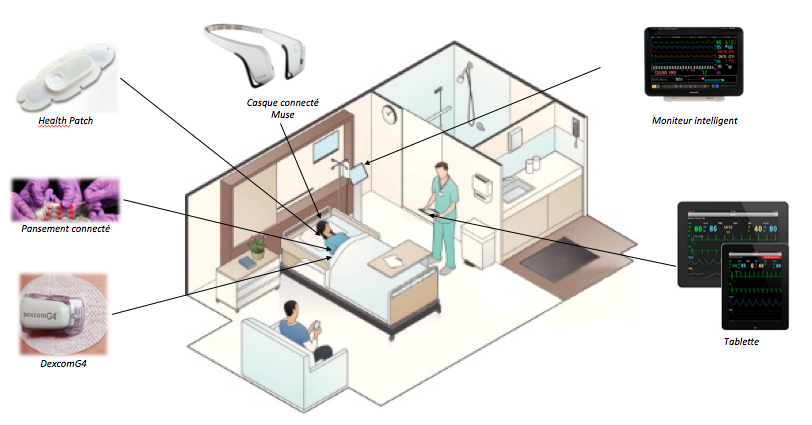
\includegraphics[width=1.1\textwidth]{Figure1.png}
	\caption{Couches Dispositifs, et Protocoles de Réseau et de Communication de notre Système}
	\label{fig:couches}
\end{figure}

Rappelons que notre sujet consiste à établir un système IoT dans le domaine Smart Health, et plus précisément dans les services de
soins intensifs des hôpitaux, afin de résoudre le problèmes de congestion et de surveillance en continu dans ces services. La Figure
\ref{fig:couches} nous permet de visualiser les choix de dispositifs et de protocoles de communication et de réseau que nous avons établis
dans le rapport précédent. Avant de commencer à décrire les différents modules dont nous aurons besoin dans notre middleware, ce que nous feront dans les section 2, 3, et 4, il est important de préciser le choix que nous avons fait concernant l’architecture générale de notre middleware. En effet, nous avons décidé de diviser notre middleware en deux couches différentes, la première étant liée au moniteur qui centralise toutes les informations des divers dispositifs présents dans la chambre du patient, et qui donc va gérer l’hétérogénéité entre les dispositifs présents dans l’environnement du patient. La seconde couche middleware est liée au Gateway de notre système, qui s’occupe de centraliser les informations de tous les moniteurs (le problème d’hétérogénéité se pose moins ici), et qui va faire le lien entre la couche de stockage et celle de liaison à la couche physique. Cette seconde couche va être celle qui permettra d’identifier les différents groupements de dispositifs à travers la connaissance des différents moniteurs intelligents.

La Figure \ref{fig:vueglobale} nous permet de visualiser la structure de notre système en considérant seulement les couches dispositifs, réseaux et communication, middleware, et architecture. Ainsi, dans les trois prochaines sections, notre tâche ne sera pas seulement de décrire les différents modules dont nous avons besoin dans notre middleware, mais aussi de décrire dans quelle(s) couche(s) middleware nous en avons besoin (possiblement les deux).

\begin{figure}[h!]
	\hspace*{-2.5cm}
	\centering
	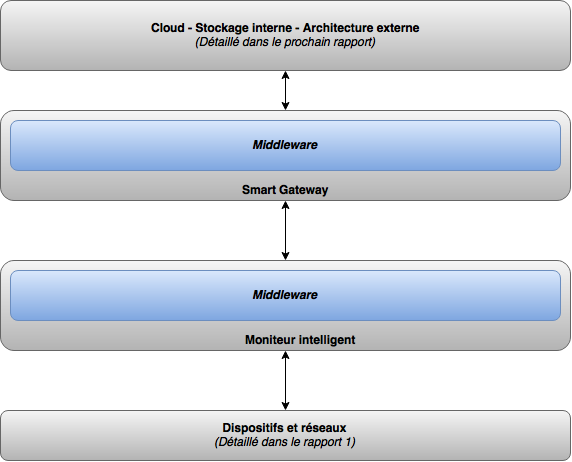
\includegraphics[width=1.4\textwidth]{Figure2.png}
	\caption{Vue Globale de notre Middleware au sein de notre Système}
	\label{fig:vueglobale}
\end{figure}


\section{Intergiciel - Middleware}
\subsection{Protocol Buffer}
Dans l'Internet des objets, tout comme dans tout système réparti, une communication entre les différentes composantes est
nécessaire. Or les données issues de divers senseurs seront probablement sous des formats variés. Il est donc obligatoire de
traduire ces données sous un autre format, qui serait le format de référence pour le reste de l'application. Cette traduction
serait à la charge du middleware afin de fournir un modèle uniforme aux futurs développeurs. Cette considération reste vraie
quel que soit l'endroit (moniteur, smartgateway) où le middleware sera déployé: la smartgateway devra récupérer des données sur le
patient depuis le cloud et les transmettre au médecin. Cette transmission nécessitera un format. De plus, il serait souhaitable
que des mécanismes soient déjà implémentés afin de générer des classes (ou tout autre abstraction utile pour le programmeur) afin
que le dit programmeur puisse directement manier ces classes sans avoir de la lecture et de l'écriture au sein de ce format.
\newline

De plus, ce format devrait être le plus léger possible. En effet, il conditionne l'apparence de ce qui circulera sur le
réseau. De ce fait, un format trop verbeux ralentirait la propagation des données et pourrait éventuellement être source de
congestion. Toutefois, ce format doit aussi être extensible. On veut pouvoir ajouter de nouvelles données si on introduit un
nouveau capteur par exemple. Enfin, ce format doit être indépendant de la plateforme ou du langage utilisé.  
\newline

Pour un tel format, notre choix s'est porté pour le \textit{protocol buffer}. En effet, il remplit tous les requis spécifiés
ci-dessus, mais a de plus des propriétés non négligeable. En particulier, ce format binaire est compatible vers l'avant et vers
l'arrière et peut traiter des messages même s'ils contiennent des champs inconnus. Cette particularité permet de faire cohabiter
différentes version d'un même logiciel. Or le problème de la mise à jour dans les grands est un problème compliqué. De plus, dans
le cadre d'un hôpital, il est impensable d'arrêter tous les systèmes pour procéder à une mise à jour globale. Cette mise à jour
sera donc incrémentielle. Or, il est tout aussi impensable que deux machines n'ayant pas la même version de logiciel ne puissent
pas échanger de message. 
\newline

Pour présenter de façon succincte le \textit{protocol buffer}, on pourra dire que c'est un format développé par \textit{Google}
avec lequel chaque message est composé de clés, types et valeurs.a Où la clé est le numéro du champ dans la spécification.

Notons que lorsqu'on parle de différentes versions, il faut, pour que la compatibilité arrière soit assurée, que les anciens
champs du message ne soit pas supprimés. En revanche, l'introduction de nouveaux champs ne posera pas de problème si les protocol
buffer sont utilisés. (Les champs inconnus seraient simplement ignorés).
\newline

Par ailleurs, la taille des messages envoyés est particulièrement optimisée. Nous avons déjà dit qu'il s'agissait d'un format
binaire, mais nous avions omis de préciser que les entiers (taille, poids, âge) sont transmis via des \textit{varint}.
C'est-à-dire des entiers de tailles variables: plus l'entier est petit moins il prend de place.


\section{ Conclusion }
TODO nouvelle conclusion
%-------------------- ancienne conclusion --------------------
%-------------------------------------------------------------
%Dans le premier rapport, nous avions présenté notre solution IoT orientée Smart Health, afin de résoudre le problème de congestion des hôpitaux dans les services de soins intensifs. Plus précisément, nous avions proposé les dispositifs et les protocoles de communication et de réseau de notre solution. Enfin, nous avions abordé les enjeux liès à la QoS, et à la sécurité et la privacité de notre solution.
%\\

%Le présent rapport a permis quant à lui de présenter le rôle du middleware dans la réponse aux problématiques de congestion de l'hôpital dans les services de soins intensifs (donc dans le cadre de notre solution). Les exigences de ces dernières ont été séparées en trois catégories, à savoir les exigences fonctionnelles, non-fonctionnelles et architecturales. Afin de remplir les différentes fonctionnalités attendues du système, différents modules au sein de notre middleware ont ainsi été identifiés. Chaque module serait destiné à remplir une fonctionnalité majeure, et à respecter une ou possiblement plusieurs exigences du middleware. Par ailleurs, nous avons présenté une conception répartie pour le middleware, conception qui peut se résumer par la présence de middlewares distincts au niveau du moniteur et de la passerelle (gateway). Nous proposons des middlewares qui pourraient opérer de manière locale comme dans un hôpital, mais qui pourraient aussi être intégrés à une plateforme IoT \cite{IBM}.

%Dans ce rapport, nous avons également mis l'accent sur les considérations sécuritaires et de confidentialité, à prendre en compte lors de la conception d'un tel système, ou plus précisément d'un tel middleware.
%\\

%L'objet du prochain rapport sera d'établir et de conceptualiser l'architecture de notre solution IoT orientée Smart Health,
%incluant la manière de stocker les données dans le Cloud, et les différentes façon dont notre solution sera exploitable à travers
%une application. Ce dernier rapport résumera la conception générale de notre solution.
%-------------------- Fin ancienne conclusion --------------------
%-----------------------------------------------------------------

 

\bibliographystyle{unsrt}




\bibliography{references}




\end{document}
